\documentclass[11pt]{book}

%%%%%%%%%%%%%%Include Packages%%%%%%%%%%%%%%%%%%%%%%%%%%
\usepackage{xcolor}
\usepackage{mathtools}
\usepackage[a4paper, total={6in, 8in}, margin=1in]{geometry}
\usepackage{amsmath}
\usepackage{amssymb}
\usepackage{paralist}
\usepackage{rsfso}
\usepackage{amsthm}
\usepackage{wasysym}
\usepackage[inline]{enumitem}   
\usepackage{hyperref}
\usepackage{tocloft}
\usepackage{wrapfig}
\usepackage{titlesec}
\usepackage{colortbl}
\usepackage{stackengine} 
\usepackage{csvsimple}
\usepackage{listings}
%%%%%%%%%%%%%%%%%%%%%%%%%%%%%%%%%%%%%%%%%%%%%%%%%%%%%%%%



%%%%%%%%%%%%%%%Code%%%%%%%%%%%%%%%%%%%%%%%%%%%%%%%%%%%%%
\definecolor{codegreen}{rgb}{0,0.6,0}
\definecolor{codegray}{rgb}{0.5,0.5,0.5}
\definecolor{codepurple}{rgb}{0.58,0,0.82}
\definecolor{backcolour}{rgb}{0.95,0.95,0.92}

\lstdefinestyle{mystyle}{
    backgroundcolor=\color{backcolour},   
    commentstyle=\color{codegreen},
    keywordstyle=\color{magenta},
    numberstyle=\tiny\color{codegray},
    stringstyle=\color{codepurple},
    basicstyle=\ttfamily\footnotesize,
    breakatwhitespace=false,         
    breaklines=true,                 
    captionpos=b,                    
    keepspaces=true,                 
    numbers=left,                    
    numbersep=5pt,                  
    showspaces=false,                
    showstringspaces=false,
    showtabs=false,                  
    tabsize=2
}
%%%%%%%%%%%%%%%%%%%%%%%%%%%%%%%%%%%%%%%%%%%%%%%%%%%%%%%%




%%%%%%%%%%%%%%%Chapter Setting%%%%%%%%%%%%%%%%%%%%%%%%%%
\definecolor{gray75}{gray}{0.75}
\newcommand{\hsp}{\hspace{20pt}}
\titleformat{\chapter}[hang]{\Huge\bfseries}{\thechapter\hsp\textcolor{gray75}{$\mid$}\hsp}{0pt}{\Huge\bfseries}
%%%%%%%%%%%%%%%%%%%%%%%%%%%%%%%%%%%%%%%%%%%%%%%%%%%%%%%%

%%%%%%%%%%%%%%%%%Theorem environments%%%%%%%%%%%%%%%%%%%
\newtheoremstyle{break}
  {\topsep}{\topsep}%
  {\itshape}{}%
  {\bfseries}{}%
  {\newline}{}%
\theoremstyle{break}
\theoremstyle{break}
\newtheorem{axiom}{Axiom}
\newtheorem{thm}{Theorem}[section]
\renewcommand{\thethm}{\arabic{section}.\arabic{thm}}
\newtheorem{lem}{Lemma}[thm]
\newtheorem{prop}[lem]{Proposition}
\newtheorem{corL}{Corollary}[lem]
\newtheorem{corT}[lem]{Corollary}
\newtheorem{defn}{Definition}[corL]
\newenvironment{indEnv}[1][Proof]
  {\proof[#1]\leftskip=1cm\rightskip=1cm}
  {\endproof}
%%%%%%%%%%%%%%%%%%%%%%%%%%%%%%%%%%%%%%%%%%%%%%%%%%%%%%


%%%%%%%%%%%%%%%%%%%%%%%Integral%%%%%%%%%%%%%%%%%%%%%%%
\def\upint{\mathchoice%
    {\mkern13mu\overline{\vphantom{\intop}\mkern7mu}\mkern-20mu}%
    {\mkern7mu\overline{\vphantom{\intop}\mkern7mu}\mkern-14mu}%
    {\mkern7mu\overline{\vphantom{\intop}\mkern7mu}\mkern-14mu}%
    {\mkern7mu\overline{\vphantom{\intop}\mkern7mu}\mkern-14mu}%
  \int}
\def\lowint{\mkern3mu\underline{\vphantom{\intop}\mkern7mu}\mkern-10mu\int}
%%%%%%%%%%%%%%%%%%%%%%%%%%%%%%%%%%%%%%%%%%%%%%%%%%%%%%



\newcommand{\R}{\mathbb{R}}
\newcommand{\N}{\mathbb{N}}
\newcommand{\Z}{\mathbb{Z}}
\newcommand{\Q}{\mathbb{Q}}
\newcommand{\C}{\mathbb{C}}
\newcommand{\T}{\mathcal{T}}
\newcommand{\M}{\mathcal{M}}
\newcommand{\Symm}{\text{Symm}}
\newcommand{\Alt}{\text{Alt}}
\newcommand{\Int}{\text{Int}}
\newcommand{\Bd}{\text{Bd}}
\newcommand{\Power}{\mathcal{P}}
\newcommand{\ee}[1]{\cdot 10^{#1}}
\newcommand{\spa}{\text{span}}
\newcommand{\sgn}{\text{sgn}}
\newcommand{\degr}{\text{deg}}
\newcommand{\pd}{\partial}
\newcommand{\that}[1]{\widetilde{#1}}
\newcommand{\lr}[1]{\left(#1\right)}
\newcommand{\vmat}[1]{\begin{vmatrix} #1 \end{vmatrix}}
\newcommand{\bmat}[1]{\begin{bmatrix} #1 \end{bmatrix}}
\newcommand{\pmat}[1]{\begin{pmatrix} #1 \end{pmatrix}}
\newcommand{\rref}{\xrightarrow{\text{row\ reduce}}}
\newcommand{\txtarrow}[1]{\xrightarrow{\text{#1}}}
\newcommand\oast{\stackMath\mathbin{\stackinset{c}{0ex}{c}{0ex}{\ast}{\Circle}}}


\newcommand{\note}{\color{red}Note: \color{black}}
\newcommand{\remark}{\color{blue}Remark: \color{black}}
\newcommand{\example}{\color{green}Example: \color{black}}
\newcommand{\exercise}{\color{green}Exercise: \color{black}}

%%%%%%%%%%%%%%%%%%%%%%Roman Number%%%%%%%%%%%%%%%%%%%%%%%
\makeatletter
\newcommand*{\rom}[1]{\expandafter\@slowromancap\romannumeral #1@}
\makeatother
%%%%%%%%%%%%%%%%%%%%%%%%%%%%%%%%%%%%%%%%%%%%%%%%%%%%%%%%%

%%%%%%%%%%%%table of contents%%%%%%%%%%%%%%%%%%%%%%%%%%%%
\setlength{\cftchapindent}{0em}
\cftsetindents{section}{2em}{3em}

\renewcommand\cfttoctitlefont{\hfill\huge\bfseries}
\renewcommand\cftaftertoctitle{\hfill\mbox{}}

\setcounter{tocdepth}{2}
%%%%%%%%%%%%%%%%%%%%%%%%%%%%%%%%%%%%%%%%%%%%%%%%%%%%%%%%%


%%%%%%%%%%%%%%%%%%%%%Footnotes%%%%%%%%%%%%%%%%%%%%%%%%%%%
\newcommand\blfootnote[1]{%
  \begingroup
  \renewcommand\thefootnote{}\footnote{#1}%
  \addtocounter{footnote}{-1}%
  \endgroup
}
%%%%%%%%%%%%%%%%%%%%%%%%%%%%%%%%%%%%%%%%%%%%%%%%%%%%%%%%%

%%%%%%%%%%%%%%%%%%%%%Section%%%%%%%%%%%%%%%%%%%%%%%%%%%%%
\makeatletter
\def\@seccntformat#1{%
  \expandafter\ifx\csname c@#1\endcsname\c@section\else
  \csname the#1\endcsname\quad
  \fi}
\makeatother
%%%%%%%%%%%%%%%%%%%%%%%%%%%%%%%%%%%%%%%%%%%%%%%%%%%%%%%%%

%%%%%%%%%%%%%%%%%%%%%%%%%%%%%%%%%%%Enumerate%%%%%%%%%%%%%%
\makeatletter
% This command ignores the optional argument 
% for itemize and enumerate lists
\newcommand{\inlineitem}[1][]{%
\ifnum\enit@type=\tw@
    {\descriptionlabel{#1}}
  \hspace{\labelsep}%
\else
  \ifnum\enit@type=\z@
       \refstepcounter{\@listctr}\fi
    \quad\@itemlabel\hspace{\labelsep}%
\fi}
\makeatother
\parindent=0pt
%%%%%%%%%%%%%%%%%%%%%%%%%%%%%%%%%%%%%%%%%%%%%%%%%%%%%%%%%%


\begin{document}

	\begin{titlepage}
		\begin{center}
			\vspace*{1cm}
			\Huge \color{red}
				\textbf{Lab 11 Report}\\
			\vspace{0.5cm}			
			\Large \color{black}
				Math 391 - Introduction to Modern Physics Lab\\
				Professor Wayne Lau\\	
				University of Michigan\\
			\vspace{3cm}

			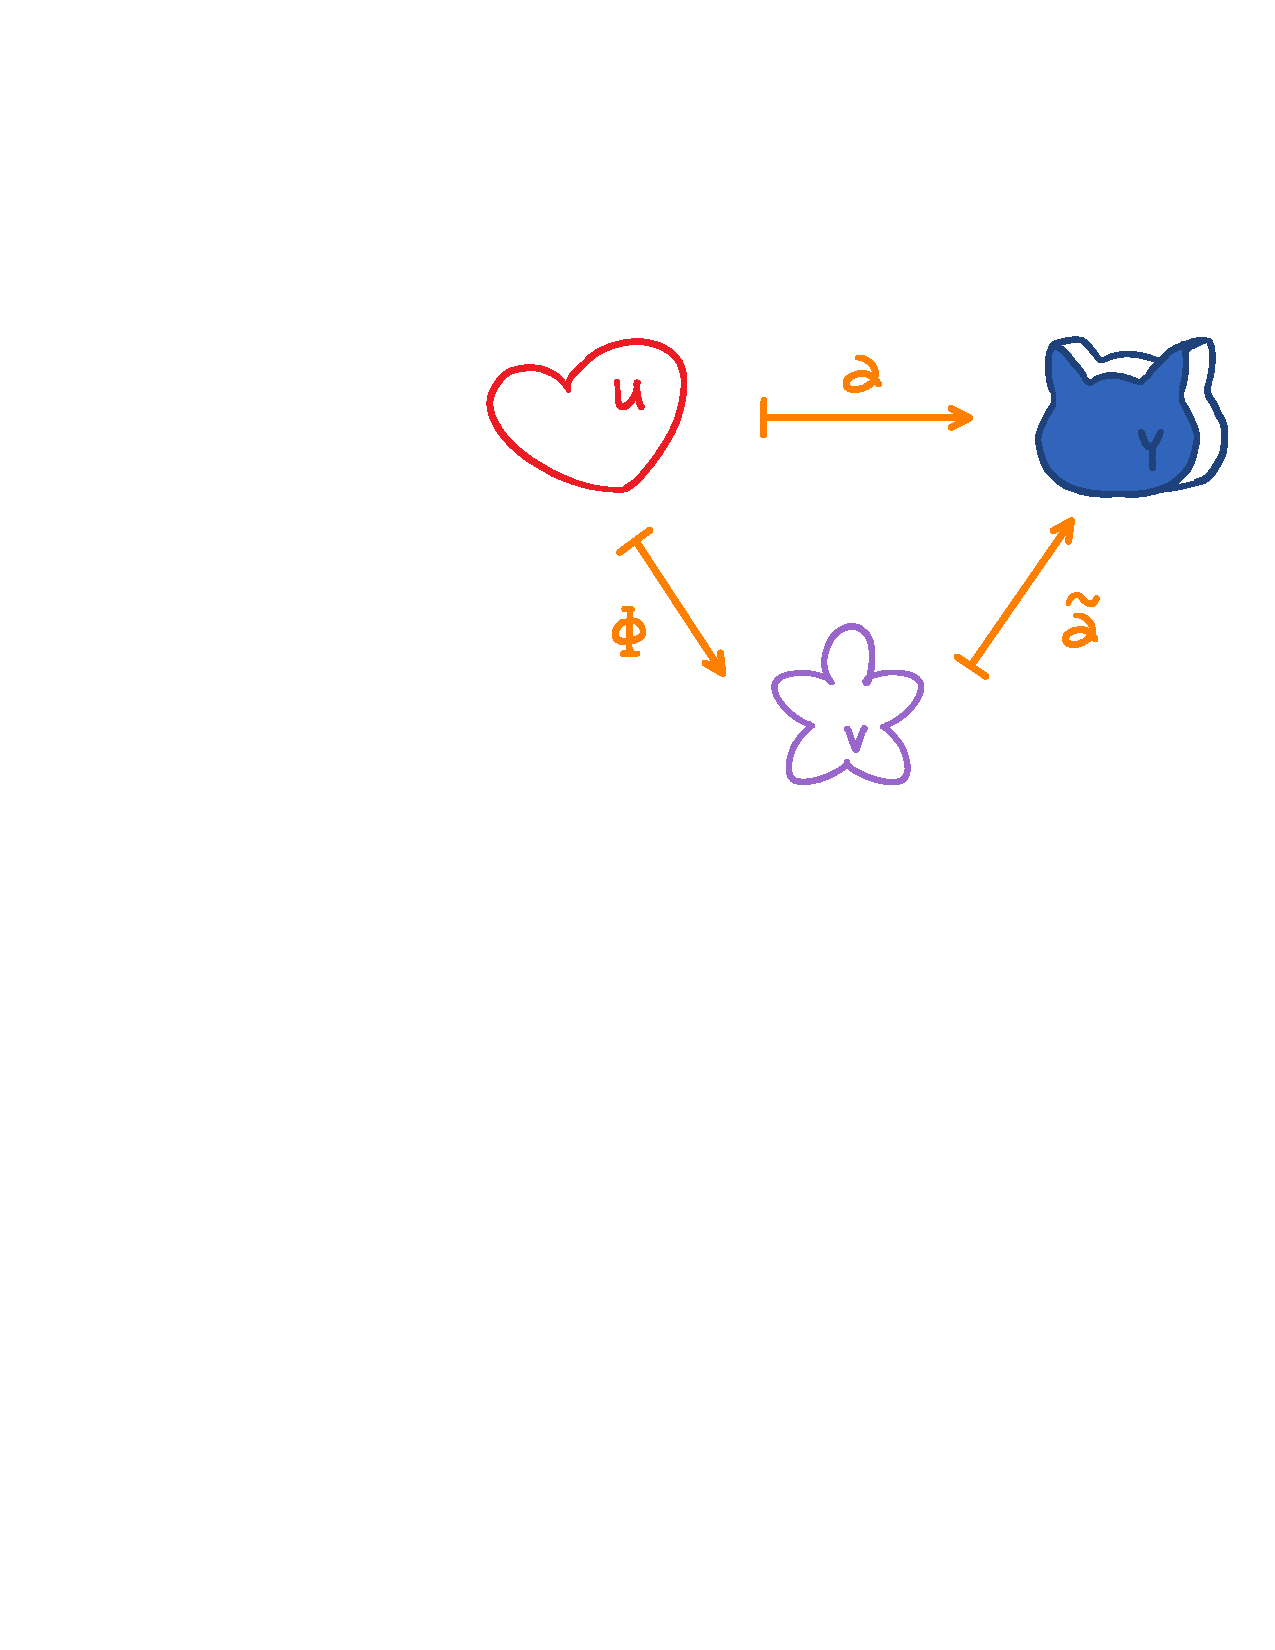
\includegraphics[scale=0.6]{Intkform.pdf}\\
			\hfill\break
			\color{gray}Figure 0. Integrating k-form over a manifold\\is independent on the use of coordinate patches\color{black}
			
			
			
			\vspace{5cm}
			\LARGE
				\textbf{Jinyan Miao}\\
				\hfill\break
				\LARGE Fall 2022\\
			\vspace{1cm}

		\vspace*{\fill}
		\end{center}			
	\end{titlepage}


\newpage
\tableofcontents
\addtocontents{toc}{~\hfill\textbf{Page}\par}


\chapter*{Lab 11 - Superconductivity}
\setcounter{chapter}{11}
\section{Introduction}
The property of superconductivity, that is having zero resistance, of many materials at extremely low temperatures has been studied in the 20th century. The discovery of superconductors was made possible by the successful liquefaction of helium in 1908 following more than a decade of effort by Heike Kamerlingh Onnes at the University of Leiden. \footnote{Akerlof, Carl W., Physics 391 Experiment 11 Lab Manual, (2018)} \\


Superconductors can be classified into two types: Type I and Type II.  For a superconductor of Type I, when it is superconducting, an external magnetic field is canceled completely in the material by the internal motion of electrons. That is, the external field does not penetrate the surface of the material until the critical field is reached and superconductivity is quenched. The phenomenon of the exclusion of the external magnetic field is called the Meissner Effect. Type II materials exhibit perfect diamagnetism up to a first critical field, but superconductivity persists above this threshold even as magnetic field lines begin to thread through the material, forming magnetic flux tubes, until a second critical field is reached at which point the sample goes normal. $^1$\\

In Lab 11 of Physics 390, we explore the properties of superconductors using two types of materials:  YBa$_2$Cu$_3$O$_7$ (YBCO) and Bi$_2$Sr$_2$Ca$_2$Cu$_3$O$_9$ (BSCCO). The two materials both have relatively high critical temperatures $T_c$. The samples are supplied as a kit from Colorado Superconductor, Inc. (CSI). In the first part of this lab, we explore the Meissner Effect. We immerse the samples in liquid nitrogen and put a small magnet on top at the center, we observe that the magnet float in the air above the superconductors. In the second part of this lab, we again immerse the two samples in liquid nitrogen and apply a DC power through the samples, and measure the resistance of the sample to estimate $T_c$.

\section{Experimental Setup}
In the first part of this lab, two 1 inches diameter superconductor disks of different materials (YBCO and BSCCO) are put on top of two inverted  12  oz. paper cups. Liquid nitrogen is then poured into the cups so that the samples are immersed in the liquid nitrogen, and the samples are cooled down below the critical temperature $T_c$. Then we put small pieces of magnets on top of the superconductors and observe what happen to the magnet.\\

In the second part of this lab, we measure the superconducting transition temperature of the two materials, YBCO and BSCCO, with 4-point probes. The calibration details of the experiment are described in the Physics 391 Lab Manual for Experiment 11. A sample is put in an 8-fluid-ounce Styrofoam coffee cup. Blue aquarium gravel has been put in the cup to maintain a relatively steady rate of change of the temperature of the sample. DC power is connected to the sample. We measure the voltage across the sample so that we can calculate the resistance of the sample, and the temperature of the sample is measured via a thermocouple. We convert the thermocouple voltage $V$ to temperature $T$ according to the following function:
\begin{align}
T = a-\sqrt{b-cV}
\end{align}
where $a=525.4425359$, $b=55647.54346$, $c=22668.77448$, and $V$ is measured in millivolt. $^1$ Once we have the setup, liquid nitrogen is poured into the cup to cool down the sample below $T_c$, the DC power is switched on and the current through the sample is maintained at around $0.45\, A$. Data is then taken. We repeat this procedure for the two samples, YBCO and BSCCO.

\section{Data Analysis}
\subsection{Observation of the Meissner Effect}
For the first part of the lab, after the samples have been cooled down below their critical values $T_c$ for which superconductivity takes place, we observe that the small magnets that are put on top of them float (airborne) above the sample surfaces, and this is due to the repulsion of the external magnetic field by the superconductors. The magnets float until the nitrogen evaporates and the samples are warmed up. There is no significant difference between what has been observed for the two samples (BSCCO and YBCO). The magnetic cubes that are put on top of the sample rotate a bit if we apply small torques on the cubes, but will soon come to a stop. We also put magnetic cylinders made with rare earth magnets, and we observe that they will rotate almost indefinitely, which is due to the differential air currents. \\

\subsection{Measuring Transition Temperature of Superconductors}
For the second part of the experiment, we first convert the measured thermocouple voltage to temperature according to (11.1), and we also convert the voltage across the samples to resistance according to $R = V/I$, where $I$ is the DC power and is fixed at $I = 0.45\, A$. The data for the two samples are presented as the followings:
\begin{center}
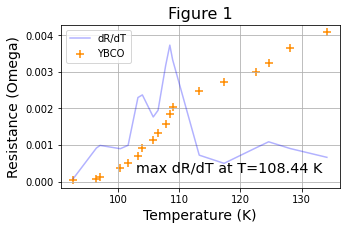
\includegraphics[scale=0.6]{1}
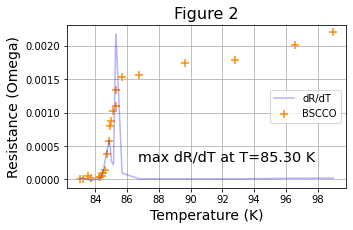
\includegraphics[scale=0.6]{2}
\end{center}
The light blue curves in Fig. 1 and Fig. 2 are computed via the gradient of data points, and are scaled by constants for visualization:
\begin{align*}
\frac{dR}{dT} = \frac{\Delta R}{\Delta T}
\end{align*}
Hence the global maxima of the blue curves represent the steepest change of resistance of the sample at a given temperature. We see that for the YBCO sample, $(dR/dT)_{max}$ occurs at $T = 108.44\, K$, hence we conclude here the transition temperature for the YBCO material is around $T_{c,\ YBCO} = 108.44\, K$. On the other hand, for the BSCCO sample, $(dR/dT)_{max}$ occurs at $T = 85.30\, K$, hence we conclude here the transition temperature for the BSCCO material is around $T_{c,\ BSCCO} = 85.30\, K$. We note here, according to the Lab Manual, the fact that these transitions are several degrees wide reflects the non-uniformity of the sample and the inability to closely control sample 
characteristics. This phenomenon is reflected by our data sets for both samples as shown in Fig. 1 and Fig 2, where we see that the transition for YBCO ranges from around 100 K to around 110 K. For the BSCCO, the transition ranges from 84 K to 86 K. Since we only have one set of data for each sample, error analysis for $T_c$ is impracticable in this experiment. In the future, we might want to repeat the procedure several times for each sample in order to get a better estimation for $T_c$. Also, notice that the resistances of the samples are nearly zero for $T<T_c$ as the measured $V$ across the samples are nearly zero. This confirms that the samples exhibit superconductivity at low temperatures $T<T_c$ because $R = V/I$ and $I = 0.45\, A$ is constant. Note that the data sets that are used in visualization in Fig. 1 and Fig. 2 are truncated to emphasize the change in resistance across $T_c$. \\

Moreover, we see that the data points for the two samples fluctuate greatly, especially for the measurement for the YBCO sample. One factor that causes the fluctuation is that the evaporation of liquid nitrogen and the space between marbles in the cups result in an unsteady rate of temperature change in the samples. A small environmental change will cause fluctuation in the data points. As a result, one way to improve the experiment is to create a more stable, in terms of change in temperature, environment for the samples, which can be made by using materials other than marbles to surround the superconducting samples, or we can use a larger container, other than small cups, for this experiment.\\

Superconductivity has demonstrated great use in modern technology. The operation of a superconducting magnet relies heavily on the use of high-temperature superconducting materials. A superconducting magnet is made from coils of superconducting wires, which are made of high-temperature superconducting materials. The magnet must be cooled to low temperatures during operation, and hence superconducting materials with higher $T_c$ are better for making the magnet. In the magnet's superconducting state, the wire has no electrical resistance and hence can conduct more current to generate a more intense magnetic field, making the superconducting magnet better than most other electromagnets. On the other hand, superconducting magnets can be cheaper to operate because no energy is dissipated as heat in the windings. Superconducting magnets are widely used in building MRI, NMR spectrometers, fusion reactors, and so on. Superconducting materials are also used in magnetic levitation for high-speed maglev trains. In Japanese design, oval superconducting coils are placed on the train, and they interact with guideway conductors to provide suspension, guidance, and propulsion of the train.\footnote{Shi, Denglu, High-Temperature Superconducting Materials Science and Engineering, (1995)}

\section{Summary}
In Lab 11 of Physics 391, we explore the properties of superconductors. Meissner Effect is observed by placing small magnets on top of the superconductor samples, where we see that the magnets float above the samples due to the repulsion of the magnetic field. We also make resistance and temperature measurements of the superconductor samples to determine their transition temperature $T_c$. From our data, the $T_c$ is estimated to be $108.44\, K$ for YBCO, and $85.30\, K$ for BSCCO. Lastly, we analyze some sources of errors in the experiment and discuss some applications of high-temperature superconductors. 

\newpage
\section{Experiment Data}
\begin{center}
\begin{tabular}{|c|c|}
\hline
    \csvreader{ALL.csv}{}{\\
    \hline
    \csvcoli&\csvcolii}\\% specify your coloumns here
\hline  
\end{tabular}  
\end{center}


\section{Code}
The code for computing statistics of the data sets is attached.
\lstset{style=mystyle}
\lstinputlisting[language=Python]{code.py}

























\end{document}